\section{Evaluation}

\subsection{Simulation Setup}
We evaluate all receivers with Sionna~\cite{hoydis2022} for $U=2$ UEs and $B=4$ BS antennas, denoted $U\times B\equiv 2\times 4$, in the configuration of Wiesmayr et al.~\cite{wiesmayr2025realtime}: dual-polarized BS antennas with 3GPP TR 38.901 patterns~\cite{tr38901}, two omnidirectional antennas per UE with beamforming $\mathbf{v}=[1,1]^{\mathsf{T}}/\sqrt{2}$, 132 PRBs with 30\,kHz subcarrier spacing at 2.14\,GHz, modulation and coding scheme (MCS) index $i=14$ (16-QAM)~\cite[Table~5.1.3.1-1]{3gpp38214}, and PUSCH mapping type A with DMRS configuration type 1 and one additional DMRS position.

To reveal the effect of the memory, we simulate sequences of 64 consecutive slots (32\,ms) over continuously evolving channels, with 32 sequences for each of three conditions, each with a new random drop of outdoor UEs per sequence, Doppler shifts up to 400\,Hz, which corresponds to the maximum UE speed of 56\,m/s in the code release of Wiesmayr et al.~\cite{wiesmayr2025realtime}, and no path loss or shadow fading: \emph{UMi}, the 3GPP model with a fixed UE drop; \emph{channel change}, UMi with both UEs switching to a newly drawn channel at slot 33; and \emph{scheduling gaps}, UMi with a pool of four UEs, in which, in every slot, a scheduled UE is replaced with probability 0.25, the DMRS ports are redrawn with probability 0.25, and a UE pauses for up to four slots with probability 0.05.

We compare the proposed NRX with three classical baselines: LS + LMMSE, which uses LS channel estimation with linear interpolation and LMMSE detection; LMMSE + K-Best, which uses LMMSE channel estimation and K-Best detection~\cite{guo2006}; and Perf.-CSI + K-Best, which uses K-Best detection with perfect channel state information (CSI).\footnote{Covariance matrices for LMMSE channel estimation are computed per condition from separately simulated channels, and the K-Best detectors apply a list size of 64.} We also compare with the released Large NRX of Wiesmayr et al.~\cite{wiesmayr2025realtime}, trained on UMi channels only and evaluated with $N_{\mathrm{it}}\in\{2,3,8\}$; with the Large NRX retrained with $N_{\mathrm{it}}=2$, i.e., the result of our first training stage, whose validation TBLER had stopped improving and from which the proposed NRX starts; and with the proposed NRX with no memory, which has identical weights but empties the memory before every TB and thus operates on LS estimates. The LS + LMMSE and K-Best receivers are taken from the code release of Wiesmayr et al.~\cite{wiesmayr2025realtime}. All receivers use 20 belief propagation iterations for decoding.

We compute the TBLER over the TBs in slots 17 to 64, after the memory has filled, i.e., over 2{,}725 to 3{,}072 TBs per condition and SNR point. All receivers decode identical channels, payloads, and noise realizations. Except in the last tests with power control, we assume, as for DMRS bundling, that each UE keeps its phase continuous across slots, without carrier frequency offset, phase noise, or timing adjustment. As in the code release, the SNR is $E_b/N_0$.

\subsection{TBLER Performance}
Fig.~\ref{fig:tbler}(a)--(c) shows TBLER vs.\ SNR without power control. We call the SNR needed for a TBLER of 10\% the required SNR. Cutting the Large NRX from $N_{\mathrm{it}}=8$ to $N_{\mathrm{it}}=2$ costs more than 1\,dB in all three conditions, and retraining it with $N_{\mathrm{it}}=2$ recovers about half a dB. The proposed NRX requires 0.51 to 0.81\,dB less than this retrained Large NRX, from which it differs only by the pilot memory and the channel filter. It also outperforms the Large NRX with $N_{\mathrm{it}}=3$ in all three conditions, by 0.28 to 0.73\,dB, and stays within 0.20\,dB of the Large NRX with $N_{\mathrm{it}}=8$, although these differences rest on only a few UEs. With the retraining, the pilot memory and the channel filter thus substitute for more than one CGNN iteration, without trained weights.

The proposed NRX outperforms LS + LMMSE in all three conditions. LMMSE + K-Best, which requires the channel statistics, remains ahead of it for UMi and channel change, whereas the proposed NRX is ahead for scheduling gaps. Perf.-CSI + K-Best remains ahead of all other receivers.

In contrast to the waterfall curves of Wiesmayr et al.~\cite{wiesmayr2025realtime}, TBLER decreases slowly with SNR for all receivers, because with a fixed beamformer and no power control, some UEs have low channel power; after the channel change, the new channel of one UE is about 18\,dB weaker than the median. Against the effective SNR, i.e., the SNR plus the mean power of the UE's effective channel over its TB in dB, the proposed NRX requires 0.58 to 0.90\,dB less than the retrained Large NRX and stays within 0.20\,dB of the Large NRX with $N_{\mathrm{it}}=8$.

\subsection{Benefit of the Pilot Memory}
Comparing the proposed NRX with its no-memory version, which operates on LS estimates, isolates the memory. The memory reduces the required SNR in all three conditions, by 0.70 to 0.78\,dB. Without its memory, the proposed NRX requires up to 0.19\,dB more than the retrained Large NRX, as its weights are trained for the refined estimates. The gain stems from the earlier slots: if the channel filter predicts every pilot from the current TB only, with its weights still fitted on the memory and with the first-order model, the proposed NRX requires 0.02 to 0.19\,dB more than with its memory emptied, i.e., on the LS estimate of the nearest pilot.

The gain of the memory grows with the Doppler shift: in effective SNR for UMi, it rises from 0.55\,dB at Doppler shifts below 50\,Hz to 0.94\,dB above 175\,Hz, as the entries mainly average the noise of the LS estimates on slow channels, whereas on fast channels the newest entry adds estimates before the first DMRS symbol of the current slot.

On two further datasets at a fixed SNR, which add TDL and UMa channels, closely spaced line-of-sight (LOS) UEs, near-far UEs, and, on one dataset, channels ray-traced with Sionna RT~\cite{hoydis2023}, the memory lowers TBLER in 16 of the 17 cases, and the proposed NRX outperforms the Large NRX with $N_{\mathrm{it}}=8$ in 6 cases, for both TDL channels and the UMa channels on both datasets, which it does not without its memory. The Large NRX with $N_{\mathrm{it}}=8$ remains ahead in 10 cases, most clearly for closely spaced LOS and near-far UEs.

The pilot memory and the channel filter do not depend on the NRX. Replacing the LMMSE channel estimation of LMMSE + K-Best, they reduce its required SNR by 0.15 to 0.43\,dB. For comparison, we extend this LMMSE estimation to the DMRS symbols of all stored TBs, up to seven, with the correlation across slots measured on separately simulated channels. This classical estimator trails the channel filter by 0.06 to 0.09\,dB for UMi and scheduling gaps and by 0.80\,dB for channel change, where it even falls 0.56\,dB behind LMMSE + K-Best, as the channel statistics cannot reveal when the channel of a UE changes.

\subsection{Power Control}
Without power control, most errors occur on UEs whose channel power stays low, and a network raises the transmit power of such UEs. We therefore also evaluate all receivers with closed-loop power control as in 5G NR~\cite{3gpp38213}: after each slot in which a UE is scheduled, the BS measures its received power, which we assume exact, and sends an accumulated transmit power control (TPC) command of $-1$, $0$, $+1$, or $+3$\,dB toward the nominal received power, at which the SNR is defined. The UE applies it in its next scheduled slot, within $-10$ to $+15$\,dB of its nominal power. Channels, payloads, noise, and receivers are those of Fig.~\ref{fig:tbler}(a)--(c), and the memory entries are not rescaled by the TPC commands.

In Fig.~\ref{fig:tbler}(d)--(f), the proposed NRX requires 0.51 to 0.71\,dB less than the retrained Large NRX and 0.36 to 0.51\,dB less than the Large NRX with $N_{\mathrm{it}}=3$. It stays within 0.17\,dB of the Large NRX with $N_{\mathrm{it}}=8$, is on par with it for UMi, and outperforms LMMSE + K-Best in all three conditions. The memory contributes 0.63 to 0.80\,dB. Power steps may also break phase continuity. With a uniformly random phase jump at every power step, the memory still contributes 0.64 to 0.81\,dB, and on each UE's first three TBs after a jump, the proposed NRX fails less often than the retrained Large NRX in all conditions. On the TB of a channel change or a phase jump, the channel filter uses no stored TB for more than 90\% of the UEs' DMRS symbols, and otherwise for less than 1\%. With a frequency offset of $\pm 0.1$\,ppm per UE, the most 3GPP allows~\cite{3gpp381011}, the proposed NRX loses less than 0.1\,dB and the retrained Large NRX about 0.15\,dB, as the channel filter tracks the rotation. With the TDD pattern DDDSU, i.e., one uplink slot every 2.5\,ms, the memory keeps more than 70\% of its gain, or at least 0.6\,dB if the eight-slot limit counts uplink slots, and the proposed NRX still leads the retrained Large NRX by at least 0.4\,dB.

\subsection{Other Modulations}
For QPSK (MCS 9) and 64-QAM (MCS 19), we train and evaluate all NRXs in the same way, starting from the released weights for each MCS; Fig.~\ref{fig:modulations} compares them at all three modulations. With QPSK and 64-QAM, the memory contributes 0.7 to 1.1\,dB, and the proposed NRX outperforms the retrained Large NRX and the Large NRX with $N_{\mathrm{it}}=3$ in all cases, with and without power control. With QPSK, it also outperforms the Large NRX with $N_{\mathrm{it}}=8$ in all cases; with 64-QAM, it stays within 0.15\,dB of it with power control, but trails it by about 0.7\,dB after scheduling gaps without power control. LS + LMMSE needs at least 0.8\,dB more with 64-QAM and 2.3\,dB more with QPSK.

\begin{figure}[!t]
\centering
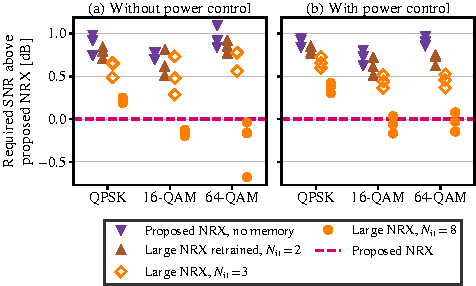
\includegraphics[width=\columnwidth]{figures/modulations_summary.pdf}
\caption{Required SNR of the stateless NRXs relative to the proposed NRX (dashed line) for QPSK, 16-QAM, and 64-QAM, without and with power control. Each marker is one test condition.}
\label{fig:modulations}
\end{figure}

\subsection{Latency}
As in Wiesmayr et al.~\cite{wiesmayr2025realtime}, we time the network from the received slot and LS estimate to the LLRs with TensorRT~10.3 in FP16 and batch size one, without decoding and host-device transfers, and export every NRX as in their code release. We report the median of 2{,}000 runs on an NVIDIA A100 GPU. The Large NRX with $N_{\mathrm{it}}=2$ takes 0.79\,ms, and each further CGNN iteration adds 0.28\,ms. Thus, $N_{\mathrm{it}}=2$ meets the 1\,ms budget, which $N_{\mathrm{it}}=3$ exceeds (1.07\,ms).

For the proposed NRX, CUDA kernels apply the channel filter before the TensorRT engine of the two CGNN iterations. The filter weights and the memory's contribution only depend on earlier slots and are computed before the slot arrives, in 0.11\,ms for both UEs. The proposed NRX takes 0.81\,ms, and the GPU work per slot including this computation is 0.91\,ms, or 0.88\,ms if it runs at the same time as the slot, so it meets the 1\,ms budget either way.